% eQoSystem, 2026 Global Quantum + AI Challenge, Phase 1
% Optional supplementary material (at most 3 pages): prior results in full,
% technical figures, and repository map. Same formatting as the proposal.
\documentclass[10pt,a4paper]{article}
\usepackage[T1]{fontenc}
\usepackage[utf8]{inputenc}
\usepackage[margin=1.8cm,top=1.7cm,bottom=1.7cm]{geometry}
\usepackage{amsmath}
\let\Bbbk\relax
\usepackage{newtxtext,newtxmath}
\usepackage{graphicx}
\usepackage{booktabs}
\usepackage{tabularx}
\usepackage{multirow}
\usepackage{xcolor}
\usepackage{microtype}
\usepackage{enumitem}
\usepackage{titlesec}
\usepackage{caption}
\usepackage{float}
\usepackage[hidelinks]{hyperref}
\usepackage{url}

\graphicspath{{figures/}}
\definecolor{eon}{RGB}{21,54,102}
\titleformat{\section}{\color{eon}\bfseries\large}{Appendix \thesection.}{0.5em}{}
\titlespacing*{\section}{0pt}{9pt plus 2pt minus 2pt}{4pt}
\renewcommand{\thesection}{\Alph{section}}
\setlength{\parskip}{2.2pt}
\setlength{\parindent}{0pt}
\setlist[itemize]{nosep,leftmargin=1.2em,topsep=1pt}
\captionsetup{font=normalsize,labelfont=bf,skip=3pt}
\renewcommand{\arraystretch}{1.08}
\renewcommand{\thetable}{A\arabic{table}}
\renewcommand{\thefigure}{A\arabic{figure}}
\pagestyle{plain}

\newcommand{\repourl}{https://github.com/AshrafBoussahi/eQoSystem-EON-GridExpansion}

\begin{document}

\begin{center}
{\color{eon}\bfseries\Large Supplementary Material}\\[3pt]
{\large Pauli Correlation Encoding for Distribution Grid Expansion Planning}\\[4pt]
Team eQoSystem, E.ON problem statement. Prior results in full, with the result
file behind each table in the public repository \url{\repourl}.
\end{center}
\vspace{2pt}\hrule\vspace{4pt}

Every number below was produced before this proposal was written and is
reproduced by the code in the repository; nothing here is projected. Tables
are grouped by the claim they support in the main text.

% ------------------------------------------------------------------ A
\section{The three-setting property, measured on a 108-qubit processor}

The claim in Section~2.2 of the proposal is operational: the number of
distinct circuits the device must execute is three, whatever the decision
count. We took two problem sizes to the Rigetti Cepheus-1-108Q through the
direct provider and submitted each in exactly three measurement settings at
1,024 shots. Table~\ref{tab:hw} is the campaign record; Figure~\ref{fig:hw}
shows the routed circuit resources and the Bell control that validates the
read-out pipeline on every edge used.

\begin{table}[h]
\centering
\caption{Measurement campaign on the Rigetti Cepheus-1-108Q. Both problem
sizes are read from three device jobs and the same 3,072 shots. Magnitude
retention is a least-squares slope against exact simulation of the same
circuit; chance-level sign agreement is 50\%. The last two rows are the
constraint that sets the depth bar in Section~3 of the proposal.}
\label{tab:hw}
\begin{tabular}{lcc}
\toprule
Quantity & $m=45$, $n=6$ & $m=105$, $n=7$ \\
\midrule
Correlation order $k$ & 2 & 3 \\
Generated gates & 59 & 68 \\
Two-qubit gates after routing & 32.3 & 40.7 \\
Depth after routing & 58 & 81 \\
\textbf{Device jobs} & \textbf{3} & \textbf{3} \\
\textbf{Shots consumed} & \textbf{3,072} & \textbf{3,072} \\
\textbf{Correlators recovered} & \textbf{45 of 45} & \textbf{105 of 105} \\
Offline check, emitted QASM against trainer state & fidelity 1.000000000000 & correlators to $3\times10^{-12}$ \\
Bell control on device edges, signs correct & \multicolumn{2}{c}{24 of 24 (8 edges, three correlators each)} \\
Bell control, mean magnitude $\langle ZZ\rangle,\langle XX\rangle,\langle YY\rangle$ & \multicolumn{2}{c}{0.82, 0.81, 0.74 (none below 0.64)} \\
\midrule
Read-out error per qubit & 6.1\% & 6.0\% \\
Correlator magnitude retained at 59 to 68 gates & 5.1\% & 2.5\% \\
\bottomrule
\end{tabular}
\end{table}

\begin{figure}[h]
\centering
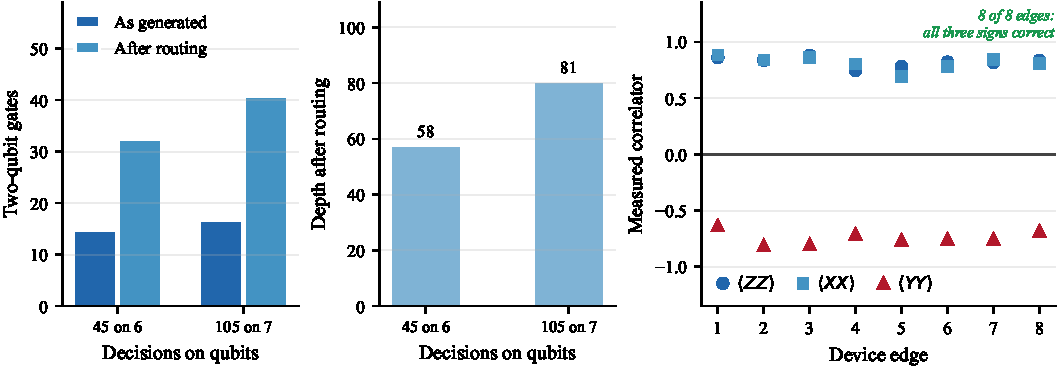
\includegraphics[width=\textwidth]{fig_hardware.pdf}
\caption{Circuit resources of the generated circuits before and after routing
onto the device lattice (left, centre), and the two-qubit Bell control on the
eight nearest-neighbour edges used (right): every edge reproduces the expected
sign of all three correlators.}
\label{fig:hw}
\end{figure}

% ------------------------------------------------------------------ B
\section{Discrete native-gate PCE circuits against variational PCE}

Section~2.3 of the proposal states that gradient-free discrete circuits lead
the variational method at low quantum budget. Table~\ref{tab:budget} is the
full record at three sizes on random 3-regular and Erd\H{o}s-R\'enyi graphs
with certified (mixed-integer) or 30-restart best-known values; the
variational arm is the brickwork ansatz of the original PCE paper trained by
Adam with parameter-shift gradients, charged $2N_p+1$ circuit executions per
step as a real device would be. Every entry is a mean raw approximation ratio
(no classical post-processing) over four instances and two runs (three to
seven runs at $m=858$).

\begin{table}[h]
\centering
\caption{Mean raw approximation ratio at matched circuit-execution budgets.
The discrete search leads at 5,000 and 20,000 executions at every size; the
variational method overtakes above $10^4$ to $10^5$ and reaches its final
value at 15 to 30 times the budget. The last column is the median correlator
magnitude, which governs shot robustness.}
\label{tab:budget}
\begin{tabular}{llccccc}
\toprule
$m$ ($n$) & Method & @5k & @20k & @100k & Final (budget) & Median $|c|$ \\
\midrule
60 (6) & Discrete PCE search & \textbf{0.885} & \textbf{0.897} & 0.897 & 0.897 (20k) & 0.11 \\
60 (6) & Variational PCE, 8 layers & 0.811 & 0.862 & 0.922 & 0.959 (414k) & 0.24 \\
60 (6) & Random circuits & 0.778 & 0.792 & & 0.792 (20k) & 0.06 \\
252 (9) & Discrete PCE search & \textbf{0.734} & \textbf{0.743} & 0.743 & 0.743 (20k) & 0.03 \\
252 (9) & Variational PCE, 8 layers & 0.665 & 0.721 & 0.801 & 0.853 (639k) & 0.13 \\
252 (9) & Random circuits & 0.670 & 0.682 & & 0.682 (20k) & 0.03 \\
858 (13) & Discrete PCE search & \textbf{0.664} & \textbf{0.673} & 0.673 & 0.673 (20k) & 0.02 \\
858 (13) & Variational PCE, 8 layers & 0.615 & 0.650 & 0.689 & 0.738 (676k) & 0.11 \\
858 (13) & Random circuits & 0.609 & 0.616 & & 0.616 (20k) & 0.02 \\
\bottomrule
\end{tabular}
\end{table}

\textbf{The smoothed term as a shot-robustness device.} The reward used by the
circuit writer combines the exact decoded objective with the $\tanh$
surrogate of the original PCE paper. At $m=252$ and 20,000 evaluations
(Table~\ref{tab:reward}) the exact objective alone produces circuits whose
correlators sit near zero and lose 13 points when read from 1,000 shots; the
surrogate restores the magnitude and most of the shot-decoded quality. This is
why the hardware campaign trains with the surrogate on.

\begin{table}[h]
\centering
\caption{Reward composition against shot-decoded quality, $m=252$, 20,000
evaluations, one instance. ``Relaxed'' is the $\tanh$ surrogate.}
\label{tab:reward}
\begin{tabular}{lcccc}
\toprule
Reward & Exact ratio & 1,000 shots & 4,000 shots & Median $|c|$ \\
\midrule
Exact objective only & 0.724 & 0.591 & 0.595 & 0.019 \\
Exact + 4 $\times$ relaxed & \textbf{0.756} & 0.688 & 0.707 & 0.072 \\
Relaxed only & 0.716 & \textbf{0.698} & \textbf{0.711} & 0.109 \\
\bottomrule
\end{tabular}
\end{table}

% ------------------------------------------------------------------ C
\section{Grid results behind Sections 2.1 and 2.4}

\textbf{Benchmark frame.} Table~\ref{tab:bench} is the classical frame around
our transmission-siting family: 80 instances on four IEEE systems with
certified optima, every arm at a matched 10,000-evaluation budget. We report
the arms that beat us as well as those we beat; the exact-match target in the
proposal (50\% on $m\le105$) is set against the 48.8\% here.

\begin{table}[h]
\centering
\caption{Storage-siting benchmark, 80 instances with certified optima, every
arm at 10,000 evaluations. ``Exact'' is the share reaching the certified
optimum; ``gap'' the mean distance from it; the last column pairs each arm
against the correlation solver on identical instances (Wilcoxon signed-rank).}
\label{tab:bench}
\begin{tabular}{lccl}
\toprule
Arm & Exact & Gap & Paired against ours \\
\midrule
Exact MIP (reference) & 100\% & 0.000 & 3.9 ms mean solve time \\
Simulated annealing & 65.0\% & 0.588 & better, $p=4.7\times10^{-4}$ \\
Unconstrained-input control & 55.0\% & 0.879 & tied, $p=0.402$ \\
Tabu search & 53.8\% & 0.712 & better, $p=0.033$ \\
\textbf{Correlation solver (ours)} & \textbf{48.8\%} & \textbf{0.984} & \\
Greedy, 20 restarts & 17.5\% & 7.977 & worse, $p=5.7\times10^{-12}$ \\
Greedy, 1 restart & 12.5\% & 12.018 & worse, $p=3.6\times10^{-13}$ \\
\bottomrule
\end{tabular}
\end{table}

\textbf{N-1 screening of decoded plans.} Every decoded plan is screened
against the complete single-outage set with a security-constrained DC optimal
power flow that may shed load at a value of lost load of 1,000~\$/MWh, with
and without the plan on identical outages (Figure~\ref{fig:resil},
Table~\ref{tab:resil}). This is the screen the PoC applies to every line
plan, so that outage risk, one of the three trade-offs in E.ON's statement, is
reported for every output.

\begin{table}[H]
\centering
\caption{N-1 screening of decoded siting plans as a data-centre load is added
at one bus: ten instances per row, every branch outaged in turn. ``Secure'' is
the share of outages served with zero shedding; ``EUE'' the expected unserved
energy over the outage set. Daggered rows: the intact power flow can no longer
serve the added load at all, so both arms are compared on identical stressed
conditions.}
\label{tab:resil}
\begin{tabular}{lccccc}
\toprule
\multirow{2}{*}{Added load} & \multicolumn{2}{c}{Secure fraction} &
\multicolumn{2}{c}{EUE (MW)} & \multirow{2}{*}{EUE cut} \\
\cmidrule(lr){2-3}\cmidrule(lr){4-5}
 & none & plan & none & plan & \\
\midrule
\multicolumn{6}{l}{\textit{IEEE-57, 80 outages per case}}\\
50 MW & 94.3\% & 96.1\% & 0.38 & 0.09 & 74.0\% \\
100 MW$^{\dagger}$ & 85.7\% & \textbf{96.6\%} & 1.43 & 0.09 & 92.8\% \\
200 MW$^{\dagger}$ & 36.4\% & \textbf{96.1\%} & 27.2 & 0.38 & 93.5\% \\
350 MW$^{\dagger}$ & 0.0\% & \textbf{62.2\%} & 171.2 & 8.5 & 95.4\% \\
\multicolumn{6}{l}{\textit{IEEE-118, 186 outages per case}}\\
100 MW & 93.6\% & 94.1\% & 1.95 & 1.62 & 17.0\% \\
200 MW$^{\dagger}$ & 0.0\% & \textbf{93.6\%} & 17.7 & 1.74 & 88.8\% \\
350 MW$^{\dagger}$ & 0.0\% & 0.0\% & 160.5 & 29.3 & 81.9\% \\
\bottomrule
\end{tabular}
\end{table}

\begin{figure}[H]
\centering
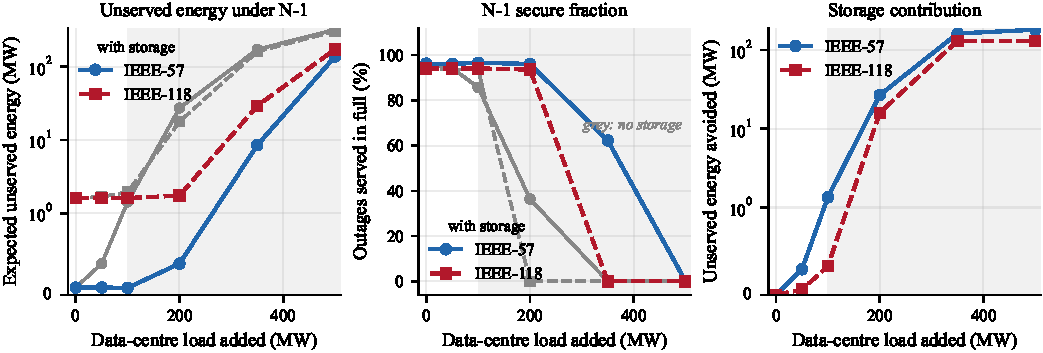
\includegraphics[width=\textwidth]{fig_r_resilience.pdf}
\caption{N-1 security of decoded plans as load is added at one bus. Coloured
curves: network with the decoded plan; grey: same network and same outages
without it. Shading marks the regime in which the intact power flow can no
longer serve the added load. Axes are symmetric-log.}
\label{fig:resil}
\end{figure}

\textbf{Extra decisions at zero qubit cost.} Adding one islanding binary per
candidate bus took the siting problem from $m=40$ to $m=44$, which the
six-qubit register (capacity 45) absorbed without a new qubit; the solver
reached the certified optimum on 60.9\% of 64 extended instances, no worse
than on the smaller problem. The same headroom argument is how conductor
tiers and switch states will share a register with line additions in the PoC.

% ------------------------------------------------------------------ D
\section{Repository map and reproduction}

The public repository holds this proposal, its figures and their generating
script, and the two code bases the PoC builds on, each with its own
reproduction commands:
\begin{itemize}
\item \texttt{qgridx/}: the grid planning package (also on PyPI as
\texttt{qgridx}), with \texttt{qgridx -{}-list} printing one command per
published table and figure, and two qBraid notebooks
(\texttt{01\_quickstart.ipynb}, \texttt{02\_hardware.ipynb}). Result files:
\texttt{results/doe\_phase3/} (benchmark, scenarios, resources, N-1,
microgrid), \texttt{results/hardware/} (Cepheus campaign).
\item \texttt{genpce/}: the Qiskit-native PCE circuit-synthesis library.
\texttt{experiments/e1\_budget\_curves.py} reproduces Table~\ref{tab:budget}
and Figure~2b of the proposal; \texttt{e2\_reward\_robustness.py} reproduces
Table~\ref{tab:reward}; \texttt{tests/} holds the 26 unit tests that check the
Walsh-Hadamard read-out against Qiskit's Pauli expectation values.
\item \texttt{proposal/}: this document and its sources.
\end{itemize}
Every experiment is seeded, resumable, and appends to CSV; the optimum of an
instance is never used by any solver, only to report approximation ratios.

\end{document}
